% Pengaturan ukuran teks dan jenis dokumen
\documentclass[11pt]{article}

% Pengaturan ukuran halaman dan margin
\usepackage[a4paper,top=30mm,left=30mm,right=20mm,bottom=20mm]{geometry}

% Pengaturan ukuran spasi
\usepackage[singlespacing]{setspace}

% Judul dokumen
\title{Proposal Pra Tugas Akhir ITS}
\author{Fathullah Auzan Setyo Laksono}

% Pengaturan format bahasa
\usepackage[indonesian]{babel}

% Pengaturan detail pada file PDF
\usepackage[pdfauthor={\@author},bookmarksnumbered,pdfborder={0 0 0}]{hyperref}

% Pengaturan jenis karakter
\usepackage[utf8]{inputenc}

% Pengaturan ukuran indentasi
\setlength{\parindent}{2em}

% Package lainnya
\usepackage{etoolbox} % Mengubah fungsi default
\usepackage{enumitem} % Pembuatan list
\usepackage{lipsum} % Pembuatan template kalimat
\usepackage{graphicx} % Input gambar
\usepackage{longtable} % Pembuatan tabel
\usepackage[table,xcdraw]{xcolor} % Pewarnaan tabel
\usepackage[numbers]{natbib} % Kutipan artikel
\usepackage{changepage} % Pembuatan teks kolom
\usepackage{multicol} % Pembuatan kolom ganda
\usepackage{multirow} % Pembuatan baris ganda
\usepackage{float}
\usepackage{outlines}

% Pengaturan format judul bab
\usepackage{titlesec}
\renewcommand{\thesection}{\arabic{section}}
\titleformat*{\section}{\normalsize\bfseries}
\titleformat*{\subsection}{\normalsize\bfseries}
\titlespacing{\section}{0ex}{3ex}{1.5ex}
\titlespacing{\subsection}{0ex}{3ex}{1.5ex}

% Isi keseluruhan dokumen
\begin{document}

  % Menonaktifkan penomoran halaman
  \pagenumbering{gobble}

  % Lembar pengesahan
  \begin{flushleft}
    % Ubah kalimat berikut sesuai dengan nama departemen dan fakultas
    \textbf{Departemen Teknik Komputer - FTEIC}\\
    \textbf{Institut Teknologi Sepuluh Nopember}\\
  \end{flushleft}
  
  \begin{center}
    % Ubah detail mata kuliah berikut sesuai dengan yang ditentukan oleh departemen
    \underline{\textbf{EC184701 - PRA TUGAS AKHIR (2 SKS)}}
  \end{center}
  
  \begin{adjustwidth}{-0.2cm}{}
    \begin{tabular}{lcp{0.7\linewidth}}
  
      % Ubah kalimat-kalimat berikut sesuai dengan nama dan NRP mahasiswa
      Nama Mahasiswa &:& Alan Luthfi \\
      Nomor Pokok &:& 07211840000063 \\
  
      % Ubah kalimat berikut sesuai dengan semester pengajuan proposal
      Semester &:& Ganjil 2021/2022 \\
  
      % Ubah kalimat-kalimat berikut sesuai dengan nama-nama dosen pembimbing
      Dosen Pembimbing &:& 1. Dr. Eko Mulyanto Yuniarno ST., MT \\
      & & 2. \\
  
      % Ubah kalimat berikut sesuai dengan judul tugas akhir
      Judul Tugas Akhir &:& \textbf{Menghitung Luas Bangun Datar pada Papan Tulis Menggunakan YOLO} \\
      %& & \textbf{Covolutional Neural Network Berbasis Citra Wajah} \\
  
      Uraian Tugas Akhir &:& \\
    \end{tabular}
  \end{adjustwidth}
  
  % Ubah paragraf berikut sesuai dengan uraian dari tugas akhir
  Papan tulis pintar memiliki potensial untuk menjadi alat pembelajaran revolusioner kedua setelah papan tulis hitam tradisional, karena papan tulis pintar yang bisa disematkan dalam ruang kelas modern bisa menggerakan sekolah ke arah mode operasi digital yang lebih terintegrasi. Pada papan tulis pintar harus memiliki fitur yang dapat membedakan papan tulis pintar dengan papan tulis biasa, karena papan tulis pintar memiliki fitur-fitur atau kegunaan lebih superior daripada papan tulis biasa. Oleh karena itu diperlukan pengembangan fitur pada papan tulis pintar. Tujuan penelitian adaah membuat program yang dapat mendeteksi bangun datar dan parameternya lalu menghitung luas bangun datar pada papan tulis pintar. Metode yang akan digunakan adalah dengan menggunakan YOLO sebagai framework pengerjaan dalam pembuatan program deteksi bangun datar dan parameternya.
  \vspace{1ex}
  
  \begin{flushright}
    % Ubah kalimat berikut sesuai dengan tempat, bulan, dan tahun penulisan
    Surabaya, Desember 2021
  \end{flushright}
  \vspace{1ex}
  
  \begin{center}
  
    \begin{multicols}{2}
  
      Dosen Pembimbing 1
      \vspace{12ex}
  
      % Ubah kalimat-kalimat berikut sesuai dengan nama dan NIP dosen pembimbing pertama
      \underline{[Dr. Eko Mulyanto Yuniarno, S.T., M.T.]} \\
      NIP. 196806011995121000
  
      \columnbreak
  
      Dosen Pembimbing 2
      \vspace{12ex}
  
      % Ubah kalimat-kalimat berikut sesuai dengan nama dan NIP dosen pembimbing kedua
      \underline{} \\
      NIP. 
  
    \end{multicols}
    \vspace{6ex}
  
    Mengetahui, \\
    % Ubah kalimat berikut sesuai dengan jabatan kepala departemen
    Kepala Departemen Teknik Komputer FTEIC - ITS
    \vspace{12ex}
  
    % Ubah kalimat-kalimat berikut sesuai dengan nama dan NIP kepala departemen
    \underline{Dr. Supeno Mardi Susiki Nugroho, S.T., M.T.} \\
    NIP. 197003131995121001
  
  \end{center}
  \newpage

  \begin{center}
    % Ubah judul
    \textbf{Menghitung Luas Bangun Datar pada Papan Tulis Menggunakan YOLO}
  \end{center}

  % Konten pendahuluan
  \section{PENDAHULUAN}

\subsection{Latar Belakang}

% Ubah paragraf-paragraf berikut sesuai dengan latar belakang dari tugas akhir
Alat pengajaran revolusioner pertama yaitu papan tulis hitam digunakan pada pengajaran dalam ruang kelas pada tahun 1801 dan memiliki dampak yang besar dalam pengajaran selama 200 tahun kedepan. Papan tulis pintar memiliki potensial untuk menjadi alat pengajaran revolusioner kedua. Seperti halnya papan tulis hitam yang menjadi bagian dari kunci ruang kelas pada abad sembilan belas dan abad dua puluh, papan tulis pintar memiliki kapabilitas untuk menjadi bagian dari kunci ruang kelas digital pada abad dua puluh satu. Meskipun relatif baru, papan tulis pintar memiliki kapasitas yang sama untuk merubah fundamental dan merevolusionerkan cara mengajar.
Dalam hal yang sama pada papan tulis hitam di zaman lampau yang merupakan teknologi yang digunakan oleh sekolah tradisional, papan tulis pintar sudah menampakkan fasilitas yang bisa digunakan oleh sekolah digital. Karena kapasitas papan tulis pintar yang bisa disematkan dalam ruang kelas modern, papan tulis pintar bisa menjadi katalis yang menggerakkan sekolah dari model tradisional berbasis kertas ke arah mode operasi digital yang lebih terintegrasi. Model sekolah tradisional berbasis kertas sudah ada dalam waktu yang cukup lama, namun kita mulai melihat pergantian pada sekolah diseluruh dunia untuk memaksimalkan potensial pembelajaran digital dan memanfaatkan keuntungan daripada kesempatan evolusi edukasi yang dibawa oleh dunia digital.
Namun perlu diingat bahwa ini adalah permulaan daripada revolusi. Tantangan yang dihadapi oleh guru dalam pengembangan pada ruang kelas digital adalah untuk melihat potensial yang tersedia lalu memanfaatkannya, dan berkolaborasi dengan rekan kerja maupun peserta didik untuk menggunakan alat pembelajaran dalam dunia digital secara efektif.



\subsection{Permasalahan}

% Ubah paragraf berikut sesuai dengan permasalahan dari tugas akhir
Pada papan tulis pintar harus memiliki fitur yang dapat membedakan papan tulis pintar dengan papan tulis biasa, karena papan tulis pintar memiliki fitur-fitur atau kegunaan lebih superior daripada papan tulis biasa. Oleh karena itu diperlukan pengembangan fitur pada papan tulis pintar. 


\subsection{Tujuan Penelitian}

% Ubah paragraf berikut sesuai dengan tujuan penelitian dari tugas akhir
Membuat program yang dapat mendeteksi bangun datar dan parameternya lalu menghitung luas bangun datar pada papan tulis menggunakan YOLO.

  % Konten tinjauan pustaka
  \section{TINJAUAN PUSTAKA}

\subsection{Deep Learning}

% Contoh penggunaan referensi dari pustaka
% Newton pernah merumuskan \citep{Newton1687} bahwa \lipsum[8]
% Contoh penggunaan referensi dari persamaan
% Kemudian menjadi persamaan seperti pada persamaan \ref{eq:FirstLaw}.

Deep learning memungkinkan model komputasi yang terdiri dari beberapa lapisan pemrosesan untuk mempelajari representasi data dengan berbagai tingkat abstraksi. Metode-metode ini telah secara dramatis meningkatkan state-of-the-art dalam pengenalan suara, pengenalan objek visual, deteksi objek dan banyak domain lainnya seperti penemuan obat dan genomik. Deep learning menemukan struktur rumit dalam kumpulan data besar dengan menggunakan algoritma backpropagation untuk menunjukkan bagaimana mesin harus mengubah parameter internalnya yang digunakan untuk menghitung representasi di setiap lapisan dari representasi di lapisan sebelumnya. Deep convolutional nets telah menghasilkan terobosan dalam pemrosesan gambar, video, ucapan, dan audio, sedangkan jaring berulang telah menyoroti data berurutan seperti teks dan ucapan.  \citep{article}

\subsection{YOLO}
YOLO (You Only Look Once) merupakan sistem deteksi objek secara waktu nyata. YOLO merupakan single CNN (Convulotional Neural Network) yang secara bersamaan memprediksi lebih dari satu bounding boxes dan kelas pada satu gambar dalam satu kali pindai. Framework ini dikembangkan oleh Redmon J., Divvala S., Girshick R., Farhadi A. arsitektur jaringannya terinspirasi dari model GoogLeNet untuk klasifikasi gambar. jaringan YOLO memiliki 24 convolutional layer diikuti dengan dua layer yang terhubung.
Saat ini, ada tiga versi YOLO yaitu YOLOv1, YOLOv2, dan YOLOv3. YOLOv2 merupakan versi yang telah dikembangkan dari YOLOv1 yang mana tetap memiliki kecepatan yang sama namun dengan penambahan batch normalization, anchor boxes dan high-resolution classifier. pada YOLOv3, fitur ektraksi yang lebih baik diperkenalkan dilanjutkan dengan perkenalan 53 convolutional layer terlatih pada ImageNet. Tingkat ketelitian YOLOv3 lebih baik dari YOLOv2 namun lebih lambat karena lebih banyak layer. \citep{Redmon_2016_CVPR}

% % input gambar
% \begin{figure} [H] \centering
%     % Nama dari file gambar yang diinputkan
%     \includegraphics[scale=0.6]{gambar/umur.png}
%     % Keterangan gambar yang diinputkan
%     \caption{Kategori umur menurut Depkes. RI (2009)}
%     % Label referensi dari gambar yang diinputkan
%     \label{fig:Umur}
% \end{figure}

\subsection{Bangun Datar}
Dalam geometri, bentuk 2D didefinisikan sebagai bangun datar yang hanya memiliki dua dimensi yaitu panjang dan lebar. Mereka tidak memiliki ketebalan apapun dan hanya dapat diukur dengan dua dimensi. Lingkaran, persegi, persegi panjang, dan segitiga adalah beberapa contoh benda dua dimensi dan bentuk-bentuk ini dapat digambar di atas kertas. Semua bentuk 2D memiliki sisi, simpul (sudut), dan sudut internal, kecuali lingkaran, yang merupakan sosok melengkung. Bentuk 2D dengan setidaknya tiga sisi lurus disebut poligon dan itu termasuk segitiga, bujur sangkar, dan segi empat.

% \subsection{Etnis}
% Kata etnis mengacu pada suatu golongan atau kelompok manusia yang anggota - anggotanya mengidentifikasikan 
% dirinya dengan sesamanya, biasanya berdasarkan garis keturunan dan adat yang dianggap sama. Identitas 
% etnis ditandai oleh pengakuan dari orang lain akan ciri khas kelompok tersebut seperti kesamaan budaya, 
% bahasa, agama, perilaku, dan ciri-ciri biologis.
% % input gambar
% \begin{figure} [H] \centering
%     % Nama dari file gambar yang diinputkan
%     \includegraphics[scale=0.6]{gambar/etnik.png}
%     % Keterangan gambar yang diinputkan
%     \caption{Macam-macam Etnik di dunia}
%     % Label referensi dari gambar yang diinputkan
%     \label{fig:Etnik}
% \end{figure}

% \subsection{Visi Komputer}
% Visi komputer adalah bidang ilmiah interdisipliner yang membahas bagaimana komputer dapat memperoleh 
% pemahaman tingkat tinggi dari gambar atau video digital. Dari perspektif teknik, bidang ini berupaya 
% mengotomatiskan tugas-tugas yang dapat dilakukan oleh sistem pengelihatan  manusia. Tugas  penglihatan 
% komputer   meliputi metode untuk memperoleh, memproses, menganalisis dan memahami gambar digital, dan 
% ekstraksi data dimensi tinggi dari dunia nyata untuk menghasilkan informasi numerik atau simbolis, 
% misalnya dalam bentuk keputusan. Pengertian dalam konteks ini berarti transformasi gambar visual 
% (input retina) menjadi deskripsi mengenai dunia sekitar yang dapat berinteraksi dengan proses pemikiran 
% lain dan memperoleh tindakan yang sesuai. Pemahaman gambar ini dapat dilihat sebagai penguraian informasi 
% simbolik dari data gambar menggunakan model yang dibangun dengan bantuan geometri, fisika, statistik, dan 
% teori pembelajaran. Sub-domain dari pengelihatan komputer meliputi rekonstruksi adegan, deteksi peristiwa, 
% pelacakan video, pengenalan objek, estimasi pose 3D, pembelajaran, pengindeksan, estimasi gerakan, dan 
% pemulihan gambar[9].

% \subsection{Machine Learning}
% Machine Learning (ML) atau Pembelajaran Mesin merupakan bagian dari Artificial Intelligence (AI) yang 
% bertujuan untuk memberi optimalisasi dalam kriteria dengan cara menganalisa sampel data yang terdahulu 
% yang sudah disimpan atau direkam untuk menghasilkan sebuah prediksi. Sehingga manusia tidak perlu 
% mengindentifikasi sebuah proses sepenuhnya, karena dengan Machine Learning, komputer mampu membuat pola 
% untuk membuat keputusan. Machine Learning melakukan training yang merupakan proses pembelajaran terhadap 
% model data yang sudah terdefinisikan ke beberapa parameter (data training) yang menghasilkan beberapa 
% pola sehingga komputer dapat melakukan proses klasifikasi berdasarkan pola atau ciri-ciri yang sudah 
% didapatkan dalam proses training. Kemudian komputer dapat memberikan sebuah prediksi pada data baru 
% selanjutnya berdasarkan hasil training. Machine Learning dapat memberi solusi dalam berbagai permasalahan
%  seperti Computer Vision (Visi Komputer), Speech Recognition (Pengenalan Suara) dan Robotics (Robotika)[10].

% \subsection{Deep Learning}
%  Deep Learning merupakan artificial neural network yang memiliki banyak layer dan synapse weight. 
%  Deep learning dapat menemukan relasi tersembunyi atau pola yang rumit antara input dan output, yang 
%  tidak dapat diselesaikan menggunakan multilayer perceptron. Keuntungan  utama  deep  learning  yaitu 
%  mampu merubah data dari nolinearly separable menjadi linearly separable melalui serangkaian transformasi 
%  (hidden layers). Selain itu, deep learning juga mampu mencari decision boundary yang berbentuk non-linier
%  , serta mengsimulasikan interaksi non-linier antar fitur. Jadi, input ditransformasikan secara 
%  non-linier sampai akhirnya pada output, berbentuk distribusi class-assignment[11].

%  \begin{figure} [H] \centering
%     % Nama dari file gambar yang diinputkan
%     \includegraphics[scale=0.6]{gambar/deeplearning.png}
%     % Keterangan gambar yang diinputkan
%     \caption{Deep Learning 4 layer}
%     % Label referensi dari gambar yang diinputkan
%     \label{fig:Deep Learning}
% \end{figure}

% \subsection{Convolutional Neural Network (CNN)}
% Convolutional Neural Network (CNN) merupakan cabang dari Multilayer Perceptron (MLP) yang digunakan untuk
% mengolah data dua dimensi. CNN memiliki kedalaman jaringan yang tinggi sehingga CNN termasuk dalam jenis
% Deep Neural Network. Perbedaan CNN dengan MLP terdapat pada neuron dimana pada MLP setiap neuron hanya
% berukuran satu dimensi, sedangkan CNN setiap neuronnya berukuran dua dimensi. Pada CNN, operasi linier
% menggunakan operasi konvolusi[12].

% \subsection{Image Processing}
% Image Processing atau Pengolahan Citra merupakan teknik dalam pemrosesan gambar dengan input berupa 
% citra dua dimensi yang bertujuan untuk menyempurnakan citra atau mendapatkan informasi yang berguna 
% untuk diolah menjadi beberapa keputusan. Dalam operasi pemrosesan citra, operasi yang sering dilakukan 
% dalam format gambar grayscale. Gambar grayscale didapatkan dari pemrosesan gambar berwarna yang 
% didekomposisi menjadi komponen merah (R), hijau (G) dan biru (B) yang diproses secara independen sebagai 
% gambar grayscale. Image Processing terbagi menjadi dalam tiga tingkatan[13]:
%     \begin{enumerate}
%         \item Low-Level Image Processing \\
%         Low-Level Image Processing merupakan operasi sederhana dalam pengolahan gambar dimana input dan 
%         output berupa gambar. Contoh: contrast enchancement dan noise reduction.
%         \item Mid-Level Image Processing \\
%         Mid-Level Image Processing merupakan operasi pengolahan gambar yang melibatkan ekstrasi atribut dari 
%         gambar input. Contoh: edges, contours dan regions.
%         \item High-Level Image Processing \\
%         High-Level Image Processing merupakan merupakan kategoriyang melibatkan pemrosesan gambar kompleks 
%         yang terkait dengan analisis dan interpretasi konten dalam sebuah keadaan untuk pengambilan keputusan.
%     \end{enumerate}

% \subsection{Digital Image}
% Digital Image merupakan fungsi dua dimensi f(x,y) yang merupakan proyeksi dari bentuk tiga dimensi kedalam 
% bentuk dua dimensi dimana x dan y merupakan lokasi elemen gambar atau piksel yang berisikan nilai. Ketika
% nilai x,y dan intensitasnya berupa diskrit, maka gambar tersebut dapat dikategorikan sebagai digital
% image. Secara matematis, digital image adalah representasi matriks dari gambar dua dimensi menggunakan
% piksel. Setiap piksel  diwakili  oleh  nilai  numerik. Untuk  gambar  grayscale,  hanya  memiliki  
% satu  nilai dengan kisaran antara 0-255.Pada Gambar 2.5, untuk gambar yang berwarna, memiliki tiga 
% nilai yang mewakili merah (R), hijau (G) dan biru (B) yang masing-masing memiliki kisaran nilai yang 
% sama antara 0-255. Jika suatu gambar hanya memiliki dua intensitas, gambar tersebut dikenal sebagai 
% binary image[13].


  % Konten metodologi
  \section{METODOLOGI}

% Ubah konten-konten berikut sesuai dengan isi dari metodologi

\subsection{Data dan Peralatan/ Data dan Alat Bantu/ Material }

% Berikut merupakan data dan perlatan yang mendukung pengerjaan Tugas Akhir ini.
\begin{itemize}
   \item [$\bullet$]Dataset berupa gambar bangun datar segitiga, persegi, persegi panjang, lingkaran, dan trapesium berjumlah 50 gambar untuk tiap bangun datar
   
    % \begin{figure} [H] \centering
    %   % Nama dari file gambar yang diinputkan
    %   \includegraphics[scale=0.2]{gambar/UTKFace.png}
    %   % Keterangan gambar yang diinputkan
    %   \caption{Dataset UTKFace}
    %   % Label referensi dari gambar yang diinputkan
    %   \label{fig:UTKFace}
    % \end{figure}

   \item [$\bullet$]Dataset berupa gambar tulisan parameter bangun datar 
    \begin{itemize}
      \item [$\bullet$]Untuk bangun datar segitiga parameternya adalah huruf A(alas) dan T(tinggi) berjumlah 50 gambar untuk tiap huruf
      \item [$\bullet$]Untuk bangun datar persegi parameternya adalah huruf S(sisi) berjumlah 50 gambar untuk tiap huruf
      \item [$\bullet$]Untuk bangun datar persegi panjang parameternya adalah huruf P(panjang) dan L(lebar) berjumlah 50 gambar untuk tiap huruf
      \item [$\bullet$]Untuk bangun datar lingkaran parameternya adalah huruf R(jari-jari) berjumlah 50 gambar untuk tiap huruf
      \item [$\bullet$]Untuk bangun datar trapesium parameternya adalah huruf S1(sisi atas), S2(sisi bawah), dan T(tinggi) berjumlah 50 gambar untuk tiap huruf
      \item [$\bullet$]Angka untuk parameter (1,2,3,4,5,6,7,8,9,0) berjumlah 50 gambar untuk tiap angka
    \end{itemize}

   \item [$\bullet$]Kamera \\
   
\end{itemize}
   

\subsection{Metodologi Penelitian}
% Metodologi yang digunakan dalam pengerjaan Tugas Akhir ini adalah sebagai berikut.
    % Contoh input gambar dengan format *.jpg
    \begin{figure} [H] \centering
      % Nama dari file gambar yang diinputkan
      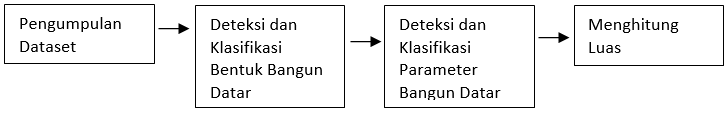
\includegraphics[scale=0.7]{gambar/Metodologi.png}
      % Keterangan gambar yang diinputkan
      \caption{Diagram blok metodologi}
      % Label referensi dari gambar yang diinputkan
      \label{fig:Metodologi}
    \end{figure}

\begin{enumerate}
   \item \textbf{Pengumpulan dataset} \\
   Pengumpulan dataset dilakukan dengan menggambar bangun datar dan parameter bangun datar pada papan tulis lalu disimpan dalam bentuk foto.
   \item \textbf{Deteksi dan Klasifikasi Bentuk Bangun Datar} \\
   Citra diproses dari kamera lalu program akan mendeteksi dan mengklasifikasi bentuk bangun datar
   \item \textbf{Deteksi dan Klasifikasi Parameter Bangun Datar} \\
   Citra diproses dari kamera lalu program akan mendeteksi dan mengklasifikasi parameter bangun datar
   \item \textbf{Menghitung Luas} \\
   Dari hasil deteksi dan klasifikasi, program akan melakukan perhitungan luas sebuah bangun datar
\end{enumerate}

  % Konten lainnya
  \section{HASIL YANG DIHARAPKAN}

Hasil yang diharapkan dalam tugas akhir ini adalah berhasil membuat program yang dapat mendeteksi bangun datar dan parameternya lalu menghitung luas bangun datar pada papan tulis dengan tingkat ketelitian yang baik.

\section{RENCANA KERJA}

% Ubah tabel berikut sesuai dengan isi dari rencana kerja
\newcommand{\w}{}
\newcommand{\G}{\cellcolor{gray}}
\begin{table}[h!]
  \begin{tabular}{|p{3.5cm}|c|c|c|c|c|c|c|c|c|c|c|c|c|c|c|c|}

    \hline
    \multirow{2}{*}{Kegiatan} & \multicolumn{16}{|c|}{Minggu} \\
    \cline{2-17} &
    1 & 2 & 3 & 4 & 5 & 6 & 7 & 8 & 9 & 10 & 11 & 12 & 13 & 14 & 15 & 16 \\
    \hline

    % Gunakan \G untuk mengisi sel dan \w untuk mengosongkan sel
    Studi Literatur &
    \G & \G & \G & \w & \w & \w & \w & \w & \w & \w & \w & \w & \w & \w & \w & \w \\
    \hline

    Pengumpulan Dataset &
    \w & \w & \w & \G & \G & \G & \w & \w & \w & \w & \w & \w & \w & \w & \w & \w \\
    \hline

    Pembuatan Model &
    \w & \w & \w & \w & \w & \G & \G & \G & \G & \G & \G & \G & \G & \w & \w & \w \\
    \hline

    % Pengujian dan Analisa &
    % \w & \w & \w & \w & \w & \w & \w & \w & \w & \w & \w & \G & \G & \G & \w & \w \\
    % \hline
    
    Pembuatan Laporan &
    \G & \G & \G & \G & \G & \G & \G & \G & \G & \G & \G & \G & \G & \G & \G & \G \\
    \hline

  \end{tabular}
\end{table}

  % Daftar pustaka
  \section{DAFTAR PUSTAKA}
  \renewcommand\refname{}
  \vspace{-2ex}
  \bibliographystyle{unsrtnat}
  \bibliography{pustaka/pustaka.bib}

\end{document}